\subsection{Quality control and tracking S/W -- database and web tracking application}
\label{sect:db}
%Need to add boxes numbers on flow-chart plot

The results of all measurements and calculations were stored in the database. Database itself represents the set of SQL tables with web interface written on PHP. Flow-chart of the database is shown on Fig.~\ref{fig:db}.

The main table named "6 bar set" is shown by the box one on Fig.~\ref{fig:db}. This table contains the set number and length of the bars in the set which are inputted manually. All other fields in this table are filled out automatically after uploading files shown in the boxes two, three and four. These files are archive outputs of analysis programs that are described in Sect.~\ref{sect:soft}.

As it mentioned above each set consists of six individual counters. Properties of the counters stored in the database are shown in box six. First two fields in box six ("bar number on label" and "bars number in order") are filled out manually, while last two fields are filled out automatically from uploaded archive file (box three).  

Each counter in its turn consists of one scintillator and two PMTs. Properties of scintillator are stored in two tables (boxes seven and eight on Fig.~\ref{fig:db}). These tables were filled out manually by workers during the construction process. Boxes nine and ten contain properties of left and right PMTs correspondingly and are filled out manually. One more quantity that is calculated in the analysis is attenuation length, it is stored in the table (see box five) that is filled out automatically when  files shown in boxes two and four were uploaded into the database. Attenuation length is the property of the scintillation material, but since PMTs are used for measurements, it's slightly different for left and right PMTs. 

Besides there is one more table (box eleven) with PMTs properties that were measured before PMTs were glued to the scintillator bar. These properties (dark current, maximum magnetic field that does not distort signal, snapshots of the signals from oscilloscope etc.) were stored in excel table and graphic files and were sorted by PMTs serial numbers. Table shown by box eleven was filled out automatically when that files were uploaded. This table is linked by PMTs serial number with tables shown by boxes nine and ten, so when tables in box nine and ten are filled out the content of the table in box eleven is automatically avaliable.

When all information about given six bar set is loaded into database one is able to print labels that should be sticked to the counter. This database is also a good tool for preliminary analysis of obtained data. For instance it allows to easely produce various plots such as time resolution versus bar length or ability to distinguish particles as function of their momentum.



\begin{figure}[]
\begin{center}
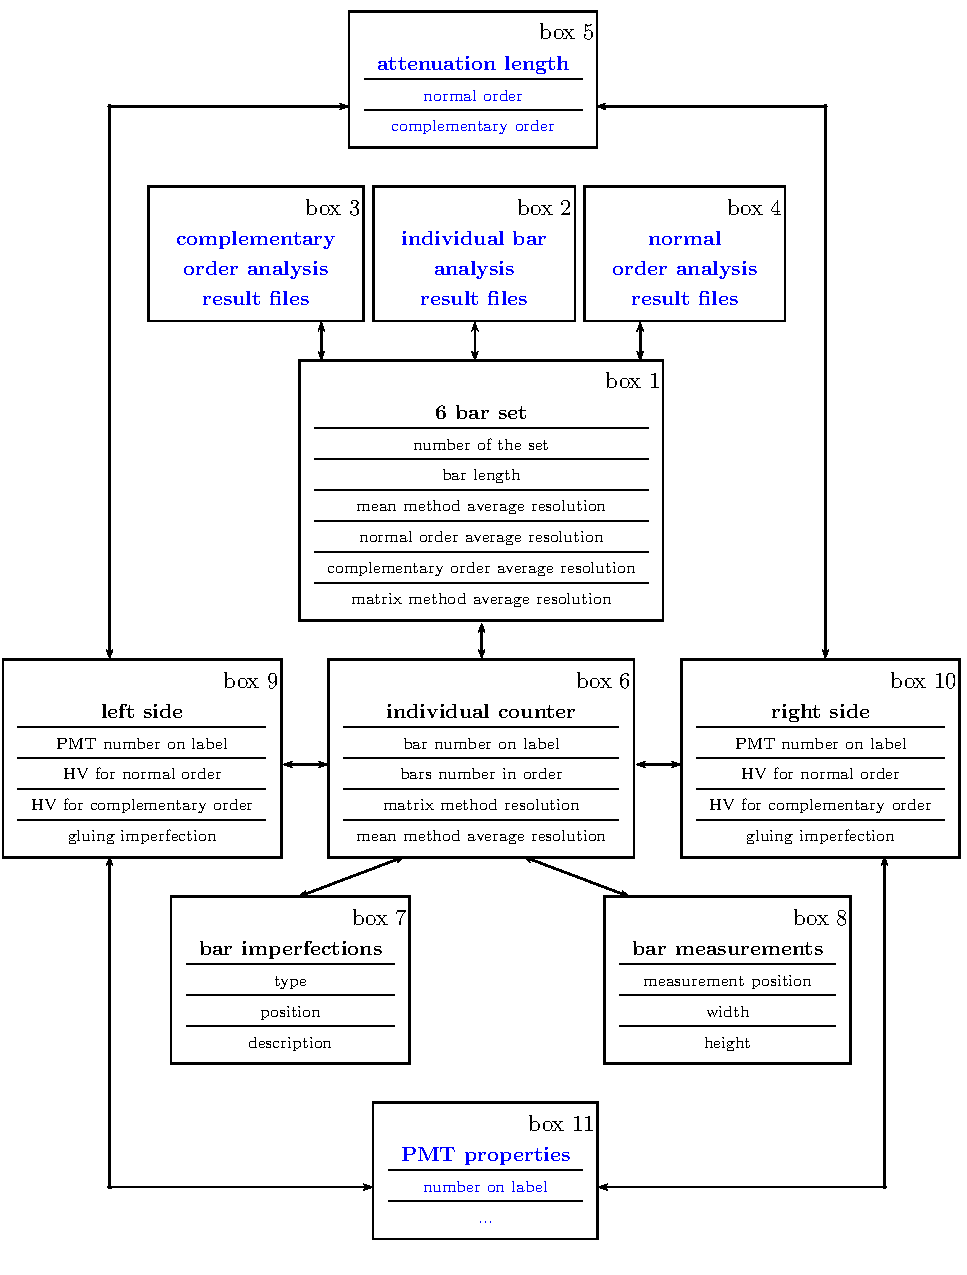
\includegraphics[width=0.9\textwidth]{gleb/fig_gleb_quality_control/db_chart.pdf}
\caption{Database structure \label{fig:db}}
\end{center}
\end{figure}




\subsection{Automated six-bar analysis software}
\label{sect:soft}
{\it Note:
note: study of required number of positional measurements at $https://clasweb.jlab.org/wiki/index.php/TOF12:20110526-fullData-SetDetails$
}
% Plot with comparison of the resolutions with different number of bins along the bar  is needed 

For simplification the analysis procedure was splitted into several stages. For the first stage converter that transforms stored data into standart root file was developed. Root file contains root tree with variables that correspond to signals from ADCs and TDCs. This approach allows in case of using different modules (for instance we used QDC, while at JLab flash ADC will be used) to modify only the converter and keep remaining analysis software unchanged.


The reason for  automated  software development is the need to repeat a lot of similar computations many times. Since the time-walk corrections are position dependent all procedures described above need to be performed in each bin along the scintillator bar. In order to determine the best bin width time resolutions were compared with expected value for various numbers of bins along the bar (see Figs. ). It turned out that the optimal width of the bin is around three cm. That means that number of bins varies from five for the shortest bars to 135 for the longest bars. 

So-called main program uses as an input root files obtained as an output of the converter. This program performs time-walk corrections (see Sect.~\ref{sect:Time-walk}) and computes resolutions for each combinations of the three bars (see Sect.~\ref{sec:six-bars}). Besides it calculates attenuation lengths and effective speeds of light (see Sect.~\ref{sect:att_speed}). As outputs program produces two files: one file with histograms that easely can be viewed by root and another archive file that can be uploaded into and processed by database (see Sect.~\ref{sect:db}). Main program need to be run twice for normal and complementary orders of the bars (see Sect.~\ref{sect:refin}).

Finally two output root files (for normal and complementary orders) from the  main program are used as inputs for the routine that computes resolutions of individual bars. This routine solves the system of linear equations mentioned in Sect.~\ref{sect:refin}.  As an output again routine has two files: root and archive which can be processed by database (Sect.~\ref{sect:db}).
